% Copyright (c) 2010 Jérémie DECOCK (http://www.jdhp.org)

\documentclass{beamer}
\usepackage[utf8]{inputenc}
\usepackage[frenchb]{babel}
\usepackage{hyperref}
\usepackage{subfigure}
%\usepackage[pdftex]{graphicx}
%\usepackage{natbib}
\usepackage{listings}
%\usepackage{algorithmic}
\usepackage{calc}


\lstset{
    basicstyle=\small,                                % print whole listing small
    keywordstyle=\color{black}\bfseries\underbar,     % underlined bold black keywords
    identifierstyle=,                                 % nothing happens
    commentstyle=\color{white},                       % white comments
    stringstyle=\ttfamily,                            % typewriter type for strings
    showstringspaces=false                            % no special string spaces
}


\hypersetup{
	pdftoolbar=true,                                          % show Acrobat’s toolbar ?
	pdfmenubar=true,                                          % show Acrobat’s menu ?
	pdffitwindow=true,                                        % page fit to window when opened
	pdftitle={},                                % title
	pdfauthor={Jérémie DECOCK},                                                                               % author
	pdfsubject={},  % subject of the document
	pdfnewwindow=true,                                                                                        % links in new window
	pdfkeywords={},                               % list of keywords
	colorlinks=true,                                          % false: boxed links; true: colored links
	linkcolor=black,                                          % color of internal links
	citecolor=black,                                          % color of links to bibliography
	filecolor=black,                                          % color of file links
	urlcolor=black                                            % color of external links
}


%\mode<presentation> {
%    \usetheme{Frankfurt}
%}

\title{Pyarm}
\author{Jérémie \bsc{Decock}}
\institute{ISIR}
\date{\today{}}

\begin{document}

\begin{frame}
\titlepage
\end{frame}

%%%%%%%%%%%%%%%%%%%%%%%%%%%%%%%%%%%%%%%

\section{Présentation des modèles}
\begin{frame}
\begin{center}
{\LARGE Présentation des modèles}
\end{center}
\end{frame}


\subsection{Présentation}

\begin{frame}
\frametitle{Présentation}
\begin{center}
        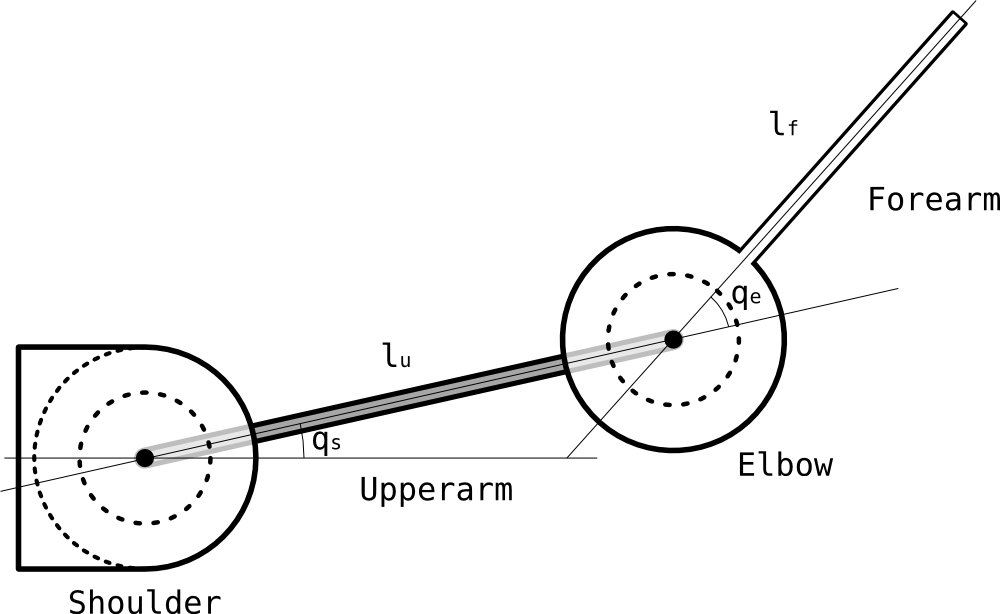
\includegraphics[width=.40\linewidth]{fig/arm}
\end{center}
\end{frame}

\begin{frame}
\frametitle{Présentation}
\begin{itemize}
    \item Bras 2D
    \item Plan horizontal (Mitrovic, Weiwei) ou vertical (Kambara)
    \item 2 membres (le bras et l'avant-bras) % ou arrière-bras ou bras supérieur
    \item 2 articulations (épaule et coude)
    \item 6 muscles~:
    \begin{enumerate}
        \item fléchisseur de l'épaule
        \item extenseur de l'épaule
        \item fléchisseur du coude
        \item extenseur du coude
        \item fléchisseur
        \item extenseur
    \end{enumerate}
\end{itemize}
Remarque : la numérotation des muscles est différente dans le modèle de Weiwei.
\end{frame}

\subsection{Les modèles étudiés}

\begin{frame}
\frametitle{Les modèles étudiés}
Trois modèles ont été étudiés~:
\begin{itemize}
    \item Katayama / Mitrovic
    \item Kambara
    \item Brown / Weiwei
\end{itemize}
\end{frame}

\subsection{Simulateur Pyarm}

\begin{frame}
\frametitle{Pyarm}
\begin{itemize}
    \item Codé en Python
    \item Implémente les 3 modèles
\end{itemize}
\begin{figure}
    \centering
    \subfigure{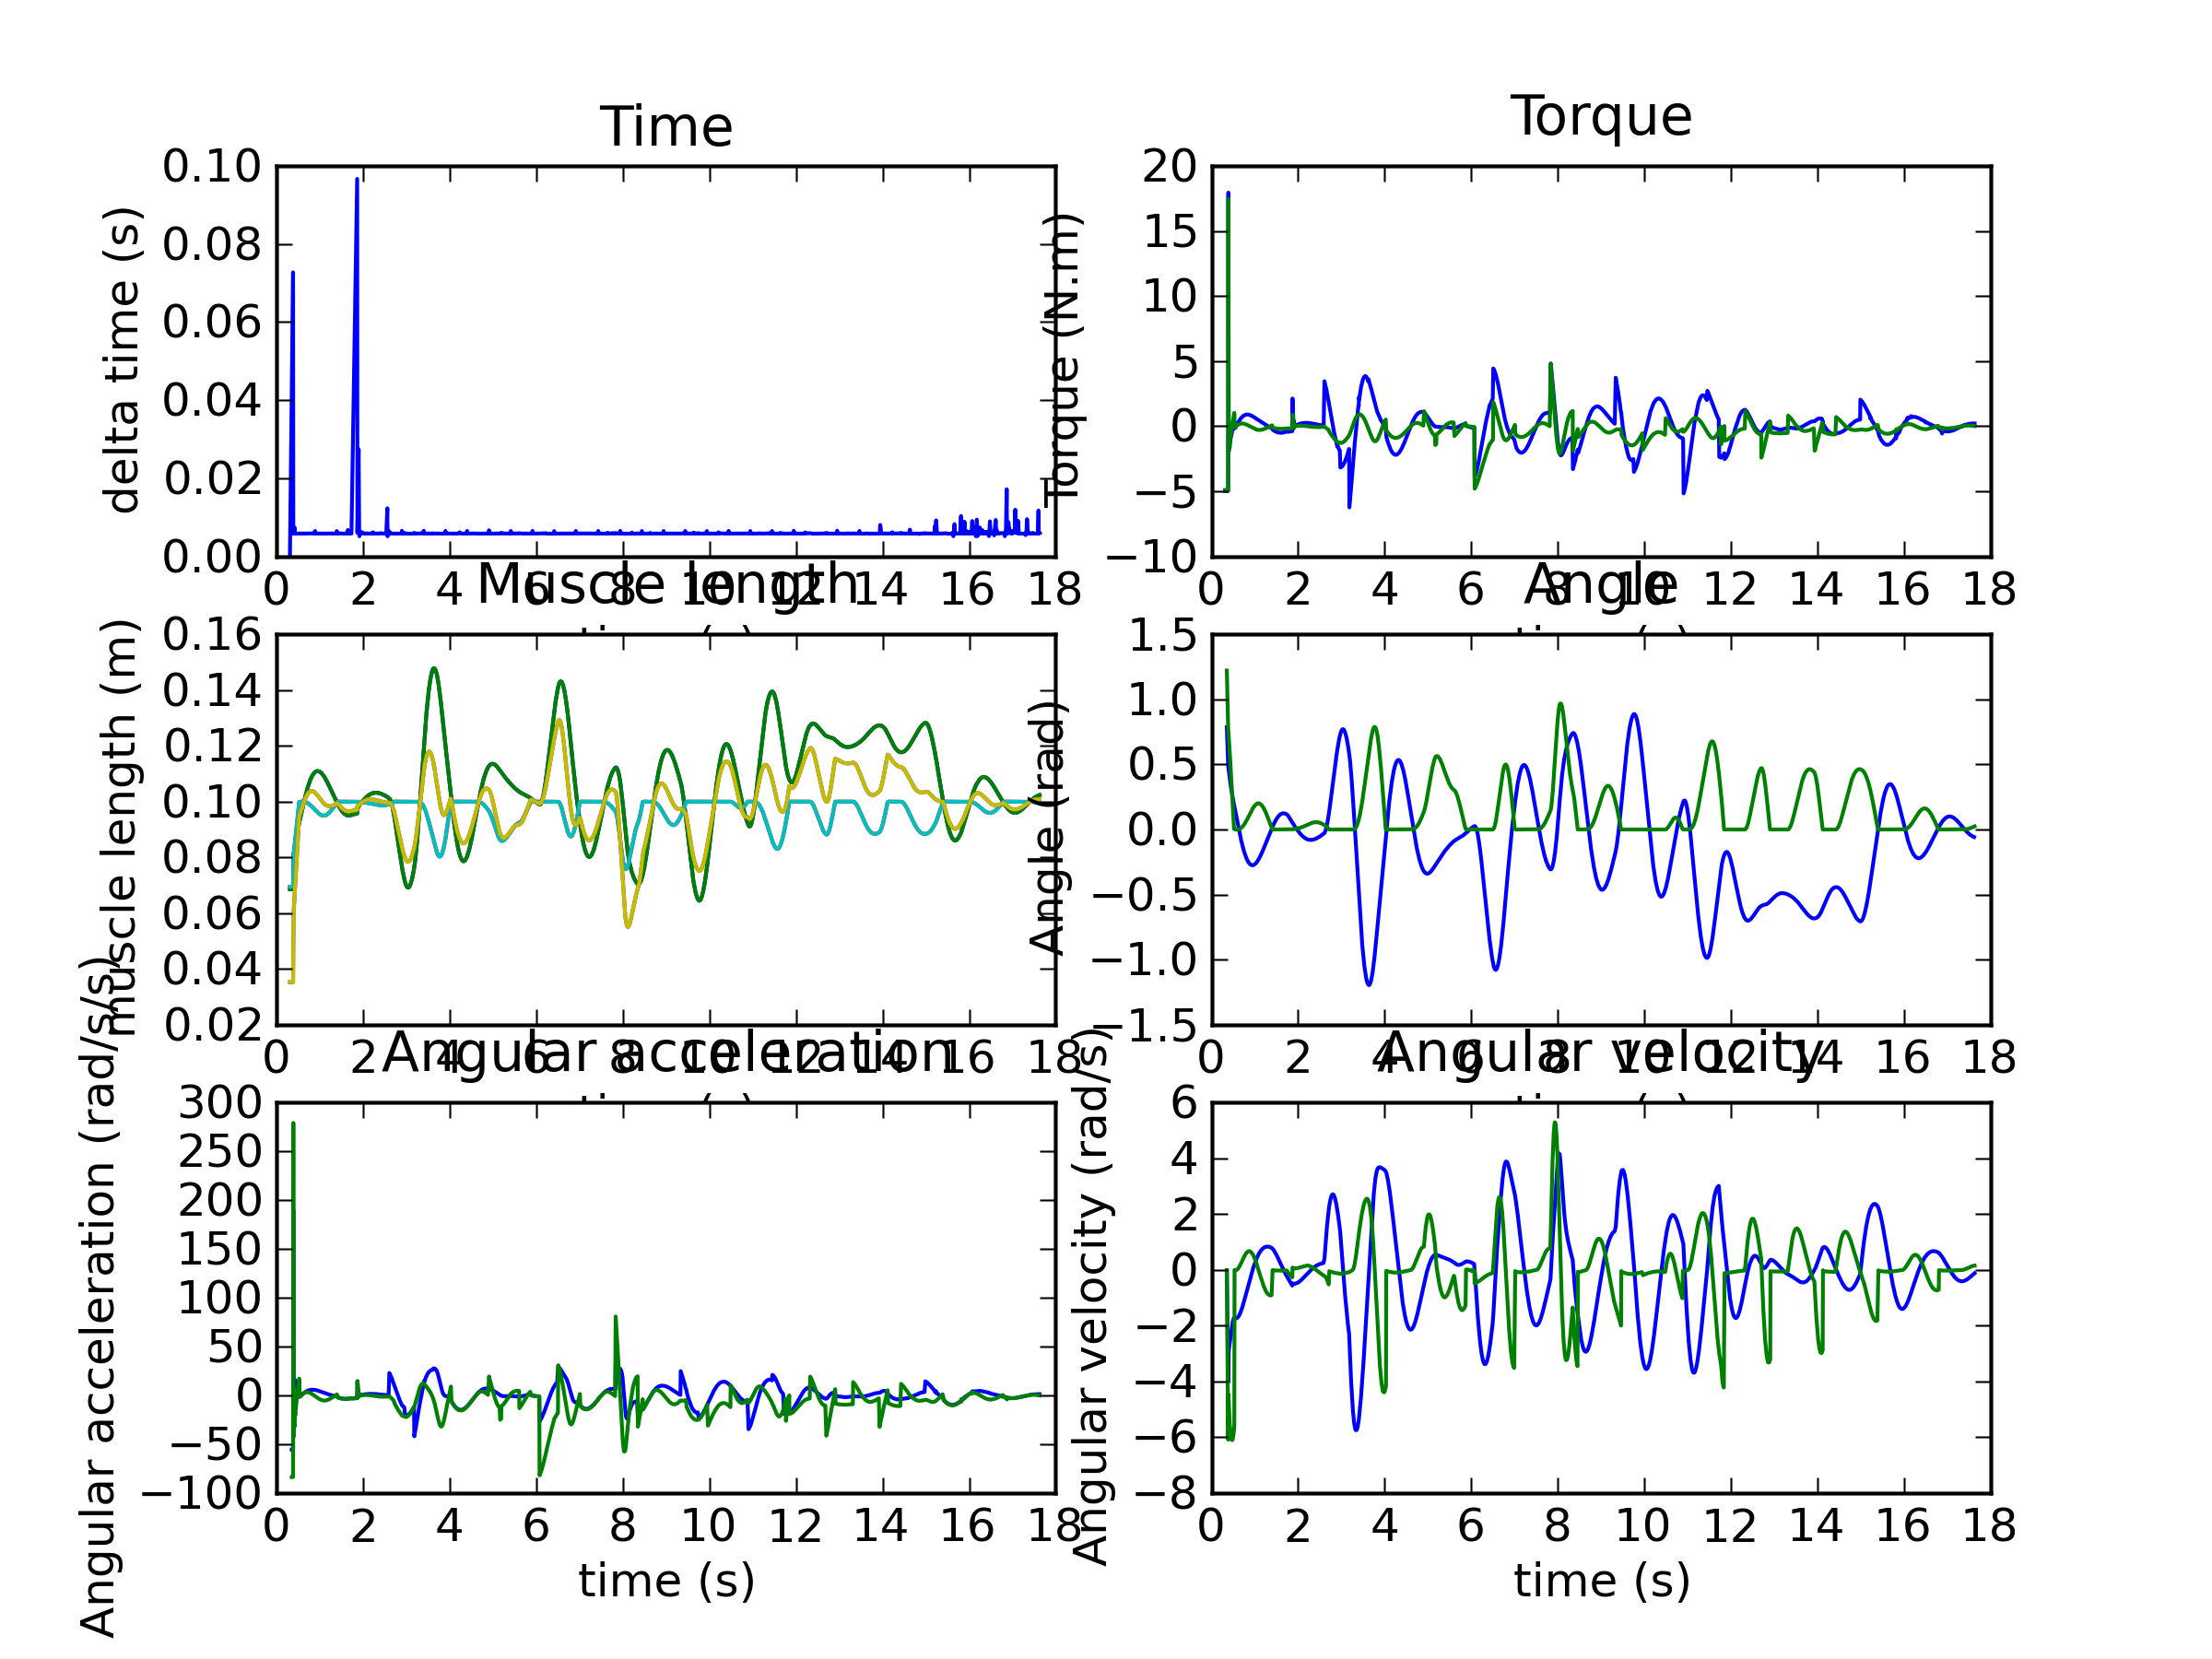
\includegraphics[width=.50\linewidth]{fig/pyarm2}}~~~
    \subfigure{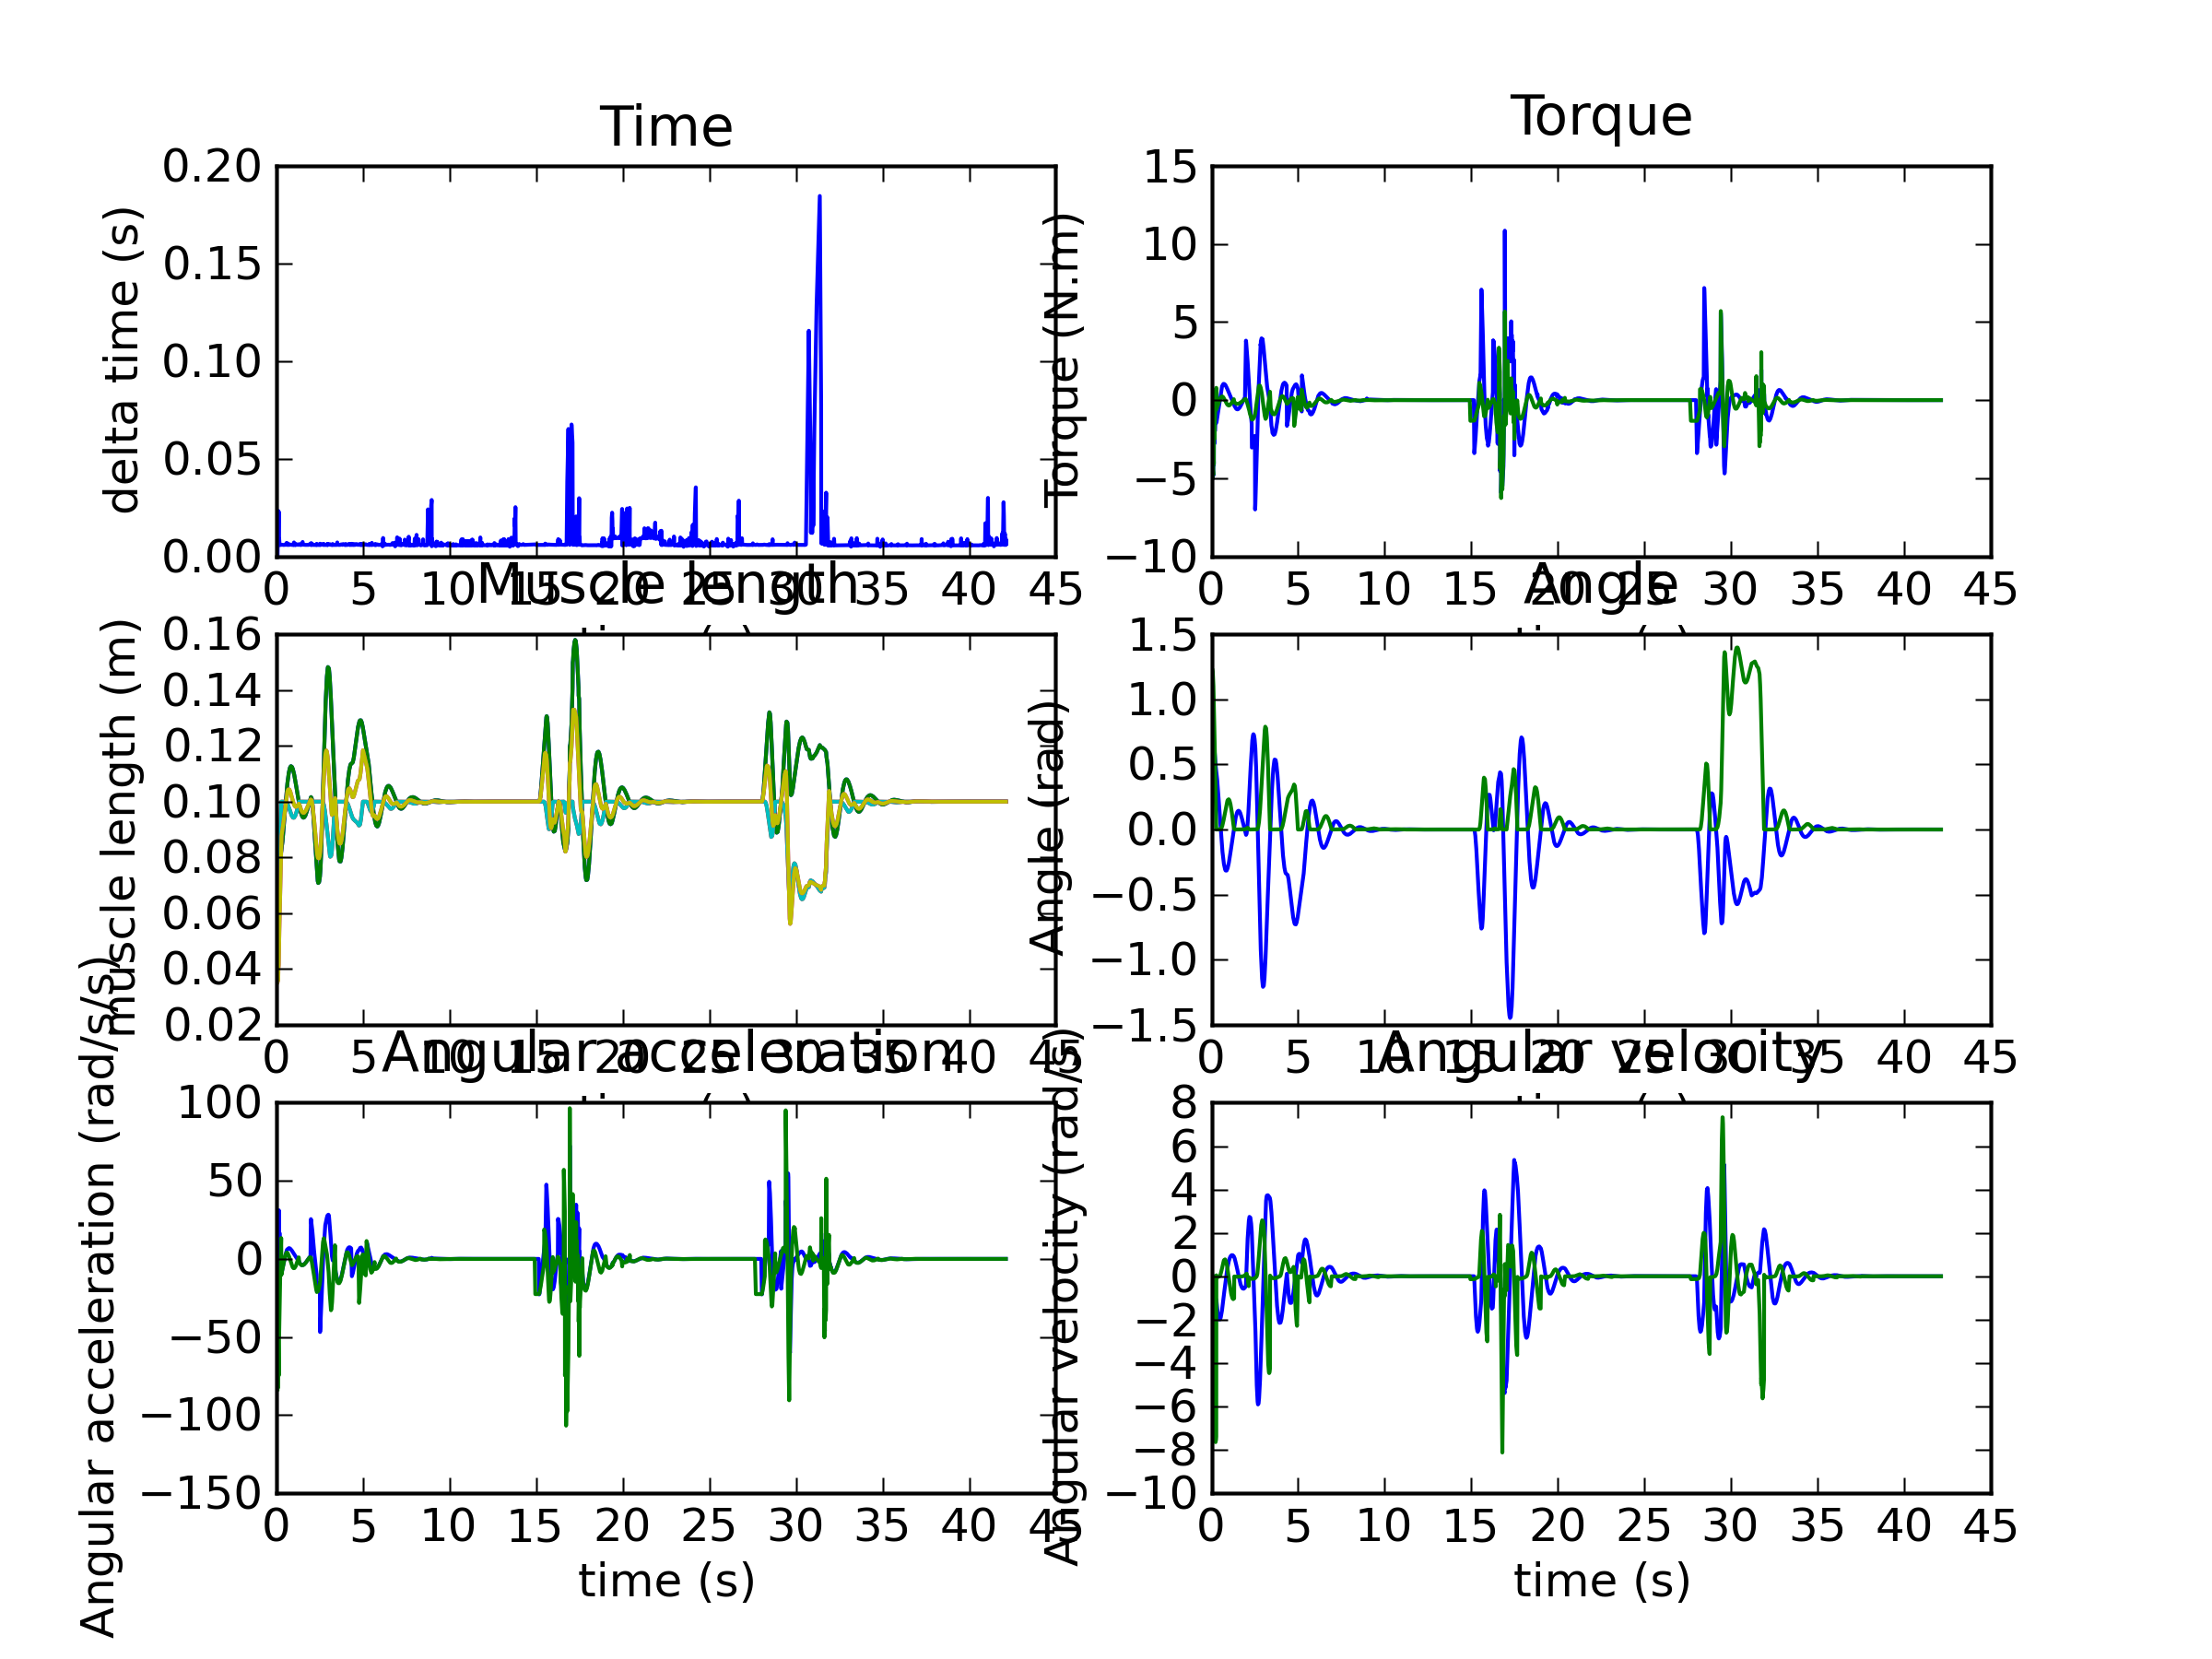
\includegraphics[width=.50\linewidth]{fig/pyarm3}}~~~
\end{figure}
\end{frame}

\begin{frame}
\frametitle{Pyarm}
Le simulateur est composé de 5 modules :
\begin{itemize}
    \item Filtre sur signal d'entrée
    \item Modèle de bras
    \begin{itemize}
        \item Cinématique
        \item Dynamique
    \end{itemize}
    \item Modèle de muscle
    \begin{itemize}
        \item Cinématique inverse
        \item Dynamique
    \end{itemize}
\end{itemize}
\end{frame}

\begin{frame}
\frametitle{Pyarm}
\begin{center}
        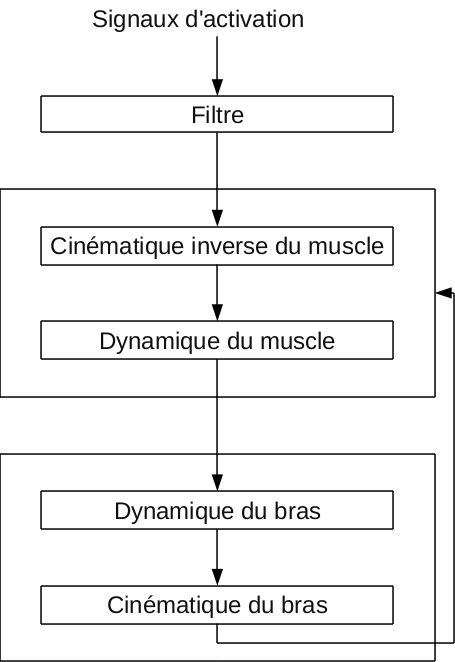
\includegraphics[width=.40\linewidth]{fig/modules}
\end{center}
\end{frame}

%%%%%%%%%%%%%%%%%%%%%%%%%%%%%%%%%%%%%%%%%%%%%%%%%%%%%%%%%%%%%%%%%%%%%%%%%%%%%%%%

\section{Cinématique inverse du muscle}
\begin{frame}
\begin{center}
{\LARGE Cinématique inverse du muscle}
\end{center}
\end{frame}

\subsection{Méthode d'Euler}

\begin{frame}
\frametitle{Cinématique inverse du muscle}
Méthode d'Euler\\
\begin{tabular}{lcl}
    $l$       & = & $l_m - A q $ \\
    $\dot{l}$ & = & $\frac{\delta l}{\delta t}$ \\
    $l_{m}$   & = & Longueur du muscle $i$ au repos pour l'angle $q = 0$ \\
\end{tabular}
\end{frame}

\begin{frame}
\frametitle{Cinématique inverse du muscle}
\begin{center}
        \includegraphics[width=.50\linewidth]{fig/moment_arm}
\end{center}
\end{frame}
    
%%%%%%%%%%%%%%%%%%%%%%%%%%%%%%%%%%%%%%%%%%%%%%%%%%%%%%%%%%%%%%%%%%%%%%%%%%%%%%%%

\section{Dynamique du muscle}
\begin{frame}
\begin{center}
{\LARGE Dynamique du muscle}
\end{center}
\end{frame}

\subsection{Mitrovic}

\begin{frame}
\frametitle{Mitrovic}
\begin{tabular}{lcl}
    $\tau$ & = & $-A^T t(l, \dot{l}, u)$ \\
    \\
    $t(l, \dot{l}, u)$        & = & $k(u) (l_r(u) - l) + b(u) \dot{l}$ \\
    \\
    $k(u)$    & = & $k_0 + k u$ \\
    $b(u)$    & = & $b_0 + b u$ \\
    $l_r(u)$  & = & $l_0 - r u$ \\
%    \\
%    $l$       & = & $l_m - A q $ \\
%    $\dot{l}$ & = & $l_m - A \dot{q} $ \\
\end{tabular}
\end{frame}

\begin{frame}
\frametitle{Mitrovic}
\begin{tabular}{lcl}
    $\tau_i$ & = & Couple total exercé sur l'articulation $i$ \\
    $A$  & = & Matrice des bras de levier \\
    $t(l, \dot{l}, u)$  & = & Tension exercée par le muscle \\
    $k(u)$ & = & Raideur du muscle \\
    $b(u)$ & = & Viscosité du muscle \\
    $l_r(u)$ & = & Longueur du muscle au repos \\
    $l$ & = & Longueur du muscle \\
    $u$ & = & Signaux d'activation du muscle \\
    $k_0$ & = & Élasticité intrinsèque \\
    $b_0$ & = & Viscosité intrinsèque \\
    $l_0$ & = & Longueur du muscle au repos \\
    $k$ & = & Coefficient de variation de l'élasticité \\
    $b$ & = & Coefficient de variation de la viscosité \\
    $r$ & = & Coefficient de variation de la longueur au repos \\
    %$l_{0i}$ & = & Longueur du muscle au repos pour l'angle $q = 0$ \\
\end{tabular}
\end{frame}

%%%%%%%%

\subsection{Kambara}

\begin{frame}
\frametitle{Kambara}
\begin{tabular}{lcl}
    $\tau$ & = & $A^T T$ \\
    \\
    $T_i$                     & = & $K_i(\tilde{u}_i) (L_i - L_i^{rest}(\tilde{u}_i)) + B_i(\tilde{u}_i) \dot{L}_i$ \\
    \\
    $K_i(\tilde{u}_i)$        & = & $k_{0i} + k_{1i} \tilde{u}_i$ \\
    $B_i(\tilde{u}_i)$        & = & $b_{0i} + b_{1i} \tilde{u}_i$ \\
    $L_i^{rest}(\tilde{u}_i)$ & = & $ l_{0i}^{rest} - l_{1i}^{rest} \tilde{u}_i$ \\
%    \\
%    $L_i$ & = & $l_{0i} - \sum_{j=1}^2 A_{i,j} q_j $ \\
\end{tabular}
\end{frame}

\begin{frame}
\frametitle{Kambara}
\begin{tabular}{lcl}
    $\tau_i$ & = & Couple total exercé sur l'articulation $i$ \\
    $A$  & = & Matrice des bras de levier \\
    $T_i$  & = & Tension exercée par le muscle $i$ \\
    $K_i(\tilde{u}_i)$ & = & Raideur du muscle $i$ \\
    $B_i(\tilde{u}_i)$ & = & Viscosité du muscle $i$ \\
    $L_i^{rest}(\tilde{u}_i)$ & = & Longueur du muscle $i$ au repos \\
    $L_i$ & = & Longueur du muscle $i$ \\
    $\tilde{u}_i$ & = & Signaux d'activation filtrés du muscle $i$ \\
    $k_{0i}$ & = & Élasticité intrinsèque \\
    $b_{0i}$ & = & Viscosité intrinsèque \\
    $l^{rest}_{0i}$ & = & Longueur du muscle $i$ au repos \\
    $k_{1i}$ & = & Coefficient de variation de l'élasticité \\
    $b_{1i}$ & = & Coefficient de variation de la viscosité \\
    $l^{rest}_{1i}$ & = & Coefficient de variation de la longueur au repos \\
    $l_{0i}$ & = & Longueur du muscle $i$ au repos pour l'angle $q = 0$ \\
\end{tabular}
\end{frame}

%%%%%%%%

\subsection{Weiwei}

\begin{frame}
\frametitle{Weiwei}
\begin{center}
        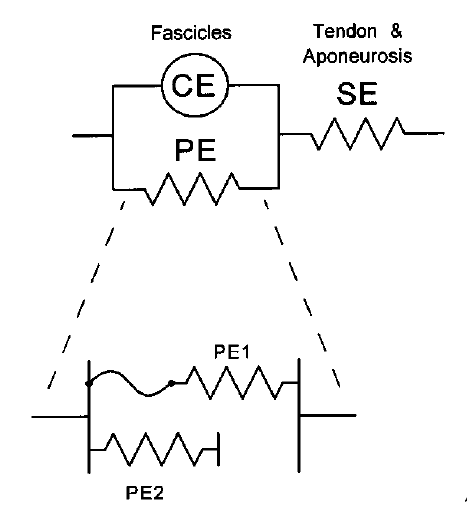
\includegraphics[width=.40\linewidth]{fig/brown}
\end{center}
\begin{tabular}{lcl}
    $CE$  & = & éléments contractiles \\
    $SE$  & = & élasticité des tendons (ignorée) \\
    $PE$  & = & élasticité du muscle \\
    $PE1$ & = & résistance à l'étirement du muscle passif \\
    $PE2$ & = & résistance à la compression du muscle actif \\
\end{tabular}
\end{frame}

\begin{frame}
\frametitle{Weiwei}
\begin{tabular}{lcl}
    $\tau$ & = & $M(q) T(a, l(q), v(q, \dot{q}))$ \\
    \\
    $T(a, l, v)$ & = & $A(a,l)(F_L(l) F_V(l,v) + F_P(l))$ \\
    $A(a, l)$    & = & $1 - \exp \left(- \left(\frac{a}{0.56 N_f(l)}\right)^{N_f(l)}\right)$ \\
    $N_f(l)$     & = & $2.11 + 4.16 \left(\frac{1}{l} - 1\right)$ \\
    $F_L(l)$     & = & $\exp \left(-\left|\frac{l^{1.93} - 1}{1.03}\right|^{1.87}\right)$ \\
    $F_V(l, v)$  & = & $\left\{ 
        \begin{array}{l}
            \frac{-5.72 - v}{-5.72 + (1.38 + 2.09 l) v}, v \leq 0 \\
            \frac{0.62 - \left(-3.12 + 4.21 l - 2.67 l^2\right) v}{0.62 + v}, v > 0 \\
        \end{array}
        \right.$ \\
    $F_P(l)$     & = & $-0.02 \exp(13.8 - 18.7 l)$ \\
\end{tabular}
\end{frame}

\begin{frame}
\frametitle{Weiwei}
\begin{tabular}{lcl}
    $M(q)$  & = & matrice des bras de levier $(a + b \cos (c q))$ \\
    $T(a, l, v)$ & = & tension exercée par le muscle \\
    $A(a, l)$    & = & relation activation-fréquence \\
%    $N_f(l)$     & = &  \\
    $F_L(l)$     & = & relation force-longueur \\
    $F_V(l, v)$  & = & relation force-vitesse \\
    $F_P(l)$     & = & force élastique du muscle \\ % TODO ???
    $a$          & = & signaux d'activation filtrés du muscle \\
    $l$          & = & longueur du muscle \\
    $v$          & = & vitesse de contraction du muscle \\
\end{tabular}
\end{frame}


%%%%%%%%%%%%%%%%%%%%%%%%%%%%%%%%%%%%%%%%%%%%%%%%%%%%%%%%%%%%%%%%%%%%%%%%%%%%%%%%

\section{Modèle du bras}
\begin{frame}
\begin{center}
{\LARGE Modèle du bras}
\end{center}
\end{frame}

%%%%%%%%

\subsection{Cas général}

\begin{frame}
\frametitle{Cas général}
Dynamique inverse : \\
$\tau = M(q)\ddot{q} + C(q, \dot{q}) + b(\dot{q}) + g(q) $ (1)\\
~\\
Dynamique :\\
(1) $\Leftrightarrow \ddot{q} = M(q)^{-1} (\tau - C(q, \dot{q}) - b(\dot{q}) - g(q)) $ \\
~\\
Légende : \\
\begin{tabular}{lcl}
    $M$      & = & matrice des moments d'inertie \\ % TODO
    $C$      & = & force de Coriolis et force centripète \\
    $b$      & = & force de viscosité et de friction \\ % TODO
    $g$      & = & force de gravité \\
    $\tau$   & = & couple total exercé sur les articulations ($N \cdot m$) \\
    $\ddot{q}$ & = & accélération angulaire ($rd \cdot s^{-2}$) \\
    $\dot{q}$ & = & vitesse angulaire ($rd \cdot s^{-1}$) \\
    $q$ & = & angle ($rd$) \\
\end{tabular}
\end{frame}

%%%%%%%%

\subsection{Mitrovic}

\begin{frame}
\frametitle{Mitrovic}
Dynamique inverse : \\
$
\begin{pmatrix}
    \tau_s \\
    \tau_e \\
\end{pmatrix}
=
\begin{pmatrix}
    I_1 + I_2 + M_2 L_1^2 + 2 M_2 L_1 L_{g2} \cos(q_e)  &  I_2 + M_2 L_1 L_{g2} \cos(q_e) \\
    I_2 + M_2 L_1 L_{g2} \cos(q_e)  &  I_2\\
\end{pmatrix}
\begin{pmatrix}
    \ddot{q}_s \\
    \ddot{q}_e \\
\end{pmatrix}
+ M_2 L_1 L_{g2} \sin(q_e)
\begin{pmatrix}
    -2 \dot{q}_e  &  -\dot{q}_e \\
    \dot{q}_s     &  0\\
\end{pmatrix}
\begin{pmatrix}
    \dot{q}_s \\
    \dot{q}_e \\
\end{pmatrix}
(2)$\\
~\\
\begin{tabular}{lcl}
    $M_j$ & = & masse du membre \\
    $L_j$ & = & longueur du membre \\
    $L_{gj}$ & = & distance séparant le centre de masse de l'articulation \\
    $I_{j}$ & = & moment d'inertie \\
\end{tabular}
~\\
(2) $\Leftrightarrow \tau = M(q)\ddot{q} + C(q, \dot{q}) \dot{q}  $ \\
~\\
Dynamique :\\
(2) $\Leftrightarrow \ddot{q} = M(q)^{-1} (\tau - C(q, \dot{q}) \dot{q}) $
\end{frame}

%%%%%%%%

\subsection{Kambara}

\begin{frame}
\frametitle{Kambara}
Dynamique inverse : \\
$
\begin{pmatrix}
    \tau_1 \\
    \tau_2 \\
\end{pmatrix}
=
\begin{pmatrix}
    M_{11}\ddot{q}_1 + M_{12}\ddot{q}_2 + h_{122}\dot{q}_2^2 + 2h_{112}\dot{q}_1\dot{q}_2 + g_1 \\
    M_{21}\ddot{q}_1 + M_{22}\ddot{q}_2 + h_{211}\dot{q}_1^2 + g_2 \\
\end{pmatrix}
(3)$\\
~\\
\begin{tabular}{lcl}
    $M_{11}$ & = & $I_1 + I_2 + m_2(l_1^2 + 2 l_1 l_{g2}\cos q_2$) \\
    $M_{12}$ & = & $I_2 + m_2l_1l_{g2}\cos q_2$ \\
    $M_{21}$ & = & $I_2 + m_2l_1l_{g2}\cos q_2$ \\
    $M_{22}$ & = & $I_2$ \\
    $h_{122}$ & = & $-m_2 l_1 l_{g2} \sin q_2$ \\
    $h_{112}$ & = & $-m_2 l_1 l_{g2} \sin q_2$ \\
    $h_{211}$ & = & $m_2 l_1 l_{g2} \sin q_2$ \\
    $g_1$ & = & $m_1 \hat{g} l_{g1} \cos q_1 + m_2 \hat{g} (l_1 \cos q_1 + l_{g2} \cos(q_1 + q_2))$ \\
    $g_2$ & = & $m_2 \hat{g} l_{g2} \cos(q_1 + q_2))$ \\
    $m_j$ & = & masse du membre \\
    $l_j$ & = & longueur du membre \\
    $l_{gj}$ & = & distance séparant le centre de masse de l'articulation \\
    $I_{j}$ & = & moment d'inertie \\
    $\hat{g}$ & = & champ de pesanteur \\
\end{tabular}\\
\end{frame}

\begin{frame}
\frametitle{Kambara}
\begin{tabular}{lcl}
    (3) & $\Leftrightarrow$ & $\tau = M(q)\ddot{q} + C(q, \dot{q}) \dot{q} + g$ \\
\end{tabular}\\
~\\
Dynamique :\\
(3) $\Leftrightarrow \ddot{q} = M(q)^{-1} (\tau - C(q, \dot{q}) \dot{q} - g) $
\end{frame}

%%%%%%%%

\subsection{Weiwei}

\begin{frame}
\frametitle{Weiwei}
Dynamique inverse :\\
$\tau = M(q)\ddot{q} + C(q, \dot{q}) + B\dot{q} $ (4)\\
~\\
\begin{tabular}{lcl}
    $M$ & = &
    $
    \begin{pmatrix}
        d1 + 2 d_2 \cos q_2  & d_3 + d_2 \cos q_2 \\
        d_3 + d_2 \cos q_2 & d_3 \\
    \end{pmatrix}
    $ \\

    $C$ & = &
    $
    \begin{pmatrix}
        -\dot{q}_2 (2 \dot{q}_1 + \dot{q}_2) \\
        \dot{q}_1^2 \\
    \end{pmatrix}
    d_2 \sin q_2
    $\\

    $B$ & = &
    $
    \begin{pmatrix}
        0.05  & 0.025 \\
        0.025 & 0.05 \\
    \end{pmatrix}
    $
\end{tabular}\\
~\\
\begin{tabular}{lcl}
    $d_1$ & = & $I_1 + I_2 + m_2 l_1^2$ \\
    $d_2$ & = & $m_2 l_1 s_2$ \\
    $d_3$ & = & $I_2$ \\
\end{tabular}\\
~\\
\begin{tabular}{lcl}
    $m_j$ & = & masse du membre \\
    $l_j$ & = & longueur du membre \\
    $s_{j}$ & = & distance séparant le centre de masse de l'articulation \\
    $I_{j}$ & = & moment d'inertie \\
\end{tabular}\\
\end{frame}

\begin{frame}
\frametitle{Weiwei}
Dynamique :\\
(4) $\Leftrightarrow \ddot{q} = M(q)^{-1} (\tau - C(q, \dot{q}) - B\dot{q}) $
\end{frame}

\subsection{Résumé}

\begin{frame}
\frametitle{Résumé}
\begin{tabular}{|c|l|}
    \hline
    Mitrovic & $\ddot{q} = M(q)^{-1} (\tau - C(q, \dot{q}) \dot{q})$ \\
    \hline
    Kambara  & $\ddot{q} = M(q)^{-1} (\tau - C(q, \dot{q}) \dot{q} - g)$ \\
    \hline
    Weiwei   & $\ddot{q} = M(q)^{-1} (\tau - C(q, \dot{q}) - B\dot{q})$ \\
    \hline
\end{tabular}
\end{frame}

%%%%%%%%%%%%%%%%%%%%%%%%%%%%%%%%%%%%%%%%%%%%%%%%%%%%%%%%%%%%%%%%%%%%%%%%%%%%%%%%

\section{Cinématique du bras}
\begin{frame}
\begin{center}
{\LARGE Cinématique du bras}
\end{center}
\end{frame}

\subsection{Méthode d'Euler}

\begin{frame}
\frametitle{Méthode d'Euler}
\begin{tabular}{lcl}
    $\dot{q}$ & = & $\delta \ddot{q} \cdot \delta t$ \\
    $q$ & = & $\delta \dot{q} \cdot \delta t$ \\
\end{tabular}
\end{frame}
    
%%%%%%%%%%%%%%%%%%%%%%%%%%%%%%%%%%%%%%%%%%%%%%%%%%%%%%%%%%%%%%%%%%%%%%%%%%%%%%%%

\section{Bibliographie}
\begin{frame}
\begin{center}
{\LARGE Bibliographie}
\end{center}
\end{frame}

\begin{frame}
\frametitle{Bibliographie}
\begin{center}
        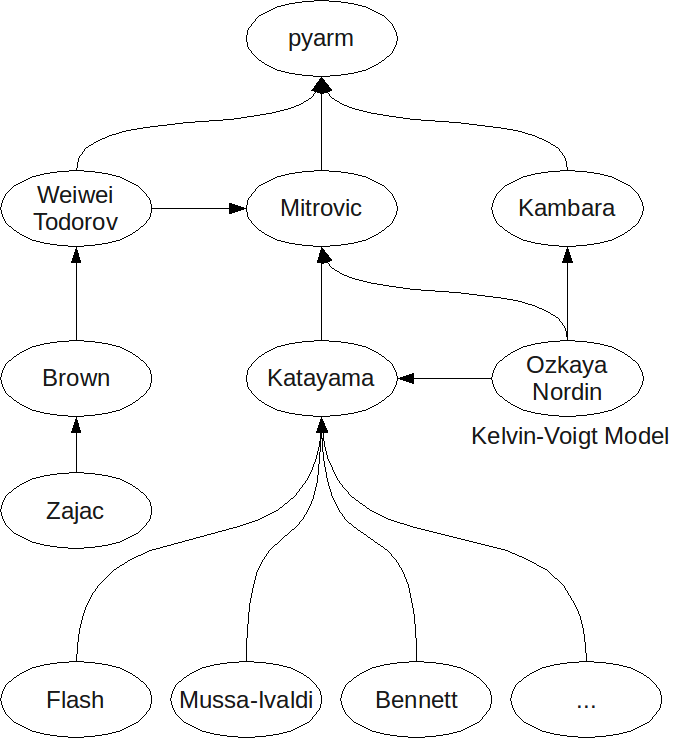
\includegraphics[width=.60\linewidth]{fig/bib}
\end{center}
\end{frame}

\end{document}
